% Created by tikzDevice version 0.12 on 2019-04-09 13:31:10
% !TEX encoding = UTF-8 Unicode
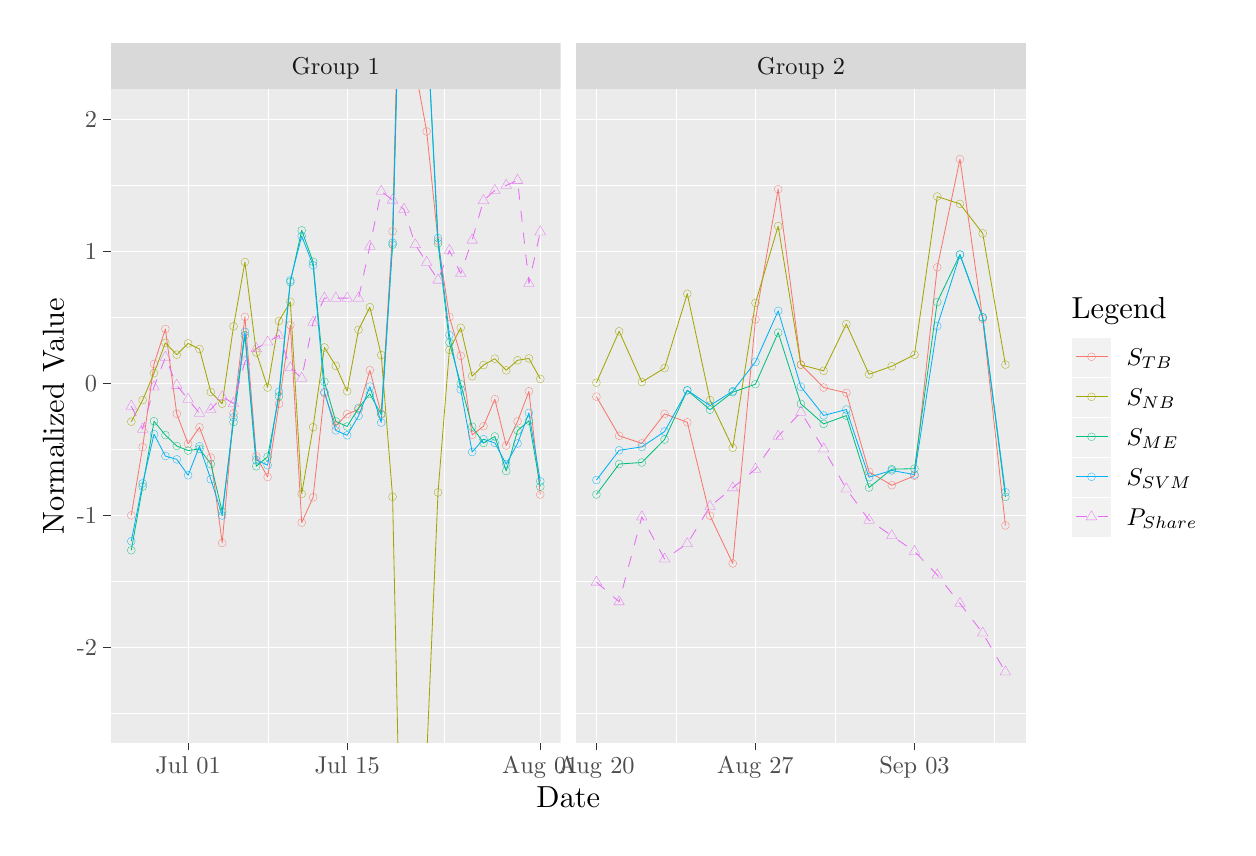
\begin{tikzpicture}[x=1pt,y=1pt]
\definecolor{fillColor}{RGB}{255,255,255}
\path[use as bounding box,fill=fillColor,fill opacity=0.00] (0,0) rectangle (433.62,289.08);
\begin{scope}
\path[clip] (  0.00,  0.00) rectangle (433.62,289.08);
\definecolor{drawColor}{RGB}{255,255,255}
\definecolor{fillColor}{RGB}{255,255,255}

\path[draw=drawColor,line width= 0.1pt,line join=round,line cap=round,fill=fillColor] (  0.00,  0.00) rectangle (433.62,289.08);
\end{scope}
\begin{scope}
\path[clip] ( 30.06, 30.73) rectangle (192.62,266.77);
\definecolor{fillColor}{gray}{0.92}

\path[fill=fillColor] ( 30.06, 30.73) rectangle (192.62,266.77);
\definecolor{drawColor}{RGB}{255,255,255}

\path[draw=drawColor,line width= 0.1pt,line join=round] ( 30.06, 41.46) --
	(192.62, 41.46);

\path[draw=drawColor,line width= 0.1pt,line join=round] ( 30.06, 89.14) --
	(192.62, 89.14);

\path[draw=drawColor,line width= 0.1pt,line join=round] ( 30.06,136.83) --
	(192.62,136.83);

\path[draw=drawColor,line width= 0.1pt,line join=round] ( 30.06,184.52) --
	(192.62,184.52);

\path[draw=drawColor,line width= 0.1pt,line join=round] ( 30.06,232.20) --
	(192.62,232.20);

\path[draw=drawColor,line width= 0.1pt,line join=round] ( 86.71, 30.73) --
	( 86.71,266.77);

\path[draw=drawColor,line width= 0.1pt,line join=round] (150.34, 30.73) --
	(150.34,266.77);

\path[draw=drawColor,line width= 0.1pt,line join=round] ( 30.06, 65.30) --
	(192.62, 65.30);

\path[draw=drawColor,line width= 0.1pt,line join=round] ( 30.06,112.99) --
	(192.62,112.99);

\path[draw=drawColor,line width= 0.1pt,line join=round] ( 30.06,160.67) --
	(192.62,160.67);

\path[draw=drawColor,line width= 0.1pt,line join=round] ( 30.06,208.36) --
	(192.62,208.36);

\path[draw=drawColor,line width= 0.1pt,line join=round] ( 30.06,256.04) --
	(192.62,256.04);

\path[draw=drawColor,line width= 0.1pt,line join=round] ( 57.97, 30.73) --
	( 57.97,266.77);

\path[draw=drawColor,line width= 0.1pt,line join=round] (115.44, 30.73) --
	(115.44,266.77);

\path[draw=drawColor,line width= 0.1pt,line join=round] (185.23, 30.73) --
	(185.23,266.77);
\definecolor{drawColor}{RGB}{248,118,109}

\path[draw=drawColor,line width= 0.3pt,line join=round] ( 37.44,112.86) --
	( 41.55,137.49) --
	( 45.66,167.56) --
	( 49.76,180.20) --
	( 53.87,149.55) --
	( 57.97,138.70) --
	( 62.08,144.66) --
	( 66.18,133.69) --
	( 70.29,102.88) --
	( 74.39,149.73) --
	( 78.50,184.58) --
	( 82.60,134.18) --
	( 86.71,126.69) --
	( 90.81,153.14) --
	( 94.92,181.60) --
	( 99.02,110.22) --
	(103.13,119.36) --
	(107.23,157.01) --
	(111.34,145.20) --
	(115.44,149.46) --
	(119.55,151.10) --
	(123.65,165.29) --
	(127.76,149.59) --
	(131.86,215.47) --
	(133.65,289.08);

\path[draw=drawColor,line width= 0.3pt,line join=round] (139.52,289.08) --
	(140.07,274.08) --
	(144.18,251.58) --
	(148.28,212.01) --
	(152.39,184.56) --
	(156.49,170.52) --
	(160.60,141.92) --
	(164.71,145.06) --
	(168.81,154.82) --
	(172.92,138.07) --
	(177.02,146.82) --
	(181.13,157.69) --
	(185.23,120.39);
\definecolor{drawColor}{RGB}{163,165,0}

\path[draw=drawColor,line width= 0.3pt,line join=round] ( 37.44,146.70) --
	( 41.55,154.50) --
	( 45.66,164.25) --
	( 49.76,175.18) --
	( 53.87,170.91) --
	( 57.97,174.99) --
	( 62.08,172.96) --
	( 66.18,157.42) --
	( 70.29,153.20) --
	( 74.39,181.17) --
	( 78.50,204.39) --
	( 82.60,171.73) --
	( 86.71,159.05) --
	( 90.81,183.12) --
	( 94.92,189.99) --
	( 99.02,120.60) --
	(103.13,144.72) --
	(107.23,173.52) --
	(111.34,166.88) --
	(115.44,157.71) --
	(119.55,179.91) --
	(123.65,188.08) --
	(127.76,170.78) --
	(131.86,119.55) --
	(134.42,  0.00);

\path[draw=drawColor,line width= 0.3pt,line join=round] (139.44,  0.00) --
	(140.07, 13.28) --
	(144.18, 25.40) --
	(148.28,121.12) --
	(152.39,172.66) --
	(156.49,180.64) --
	(160.60,163.13) --
	(164.71,167.16) --
	(168.81,169.46) --
	(172.92,165.26) --
	(177.02,168.89) --
	(181.13,169.56) --
	(185.23,162.15);
\definecolor{drawColor}{RGB}{0,191,125}

\path[draw=drawColor,line width= 0.3pt,line join=round] ( 37.44,100.23) --
	( 41.55,123.24) --
	( 45.66,146.87) --
	( 49.76,141.85) --
	( 53.87,137.91) --
	( 57.97,136.27) --
	( 62.08,136.88) --
	( 66.18,131.38) --
	( 70.29,114.21) --
	( 74.39,146.60) --
	( 78.50,177.92) --
	( 82.60,130.58) --
	( 86.71,134.04) --
	( 90.81,155.84) --
	( 94.92,197.16) --
	( 99.02,215.85) --
	(103.13,204.49) --
	(107.23,161.11) --
	(111.34,146.82) --
	(115.44,144.95) --
	(119.55,151.65) --
	(123.65,156.75) --
	(127.76,149.28) --
	(131.86,210.67) --
	(133.84,289.08);

\path[draw=drawColor,line width= 0.3pt,line join=round] (144.34,289.08) --
	(148.28,211.17) --
	(152.39,175.30) --
	(156.49,160.29) --
	(160.60,144.87) --
	(164.71,139.01) --
	(168.81,141.36) --
	(172.92,128.89) --
	(177.02,143.50) --
	(181.13,147.06) --
	(185.23,123.22);
\definecolor{drawColor}{RGB}{0,176,246}

\path[draw=drawColor,line width= 0.3pt,line join=round] ( 37.44,103.50) --
	( 41.55,124.38) --
	( 45.66,142.18) --
	( 49.76,134.29) --
	( 53.87,133.09) --
	( 57.97,127.34) --
	( 62.08,137.84) --
	( 66.18,125.89) --
	( 70.29,112.81) --
	( 74.39,148.29) --
	( 78.50,179.16) --
	( 82.60,132.86) --
	( 86.71,130.99) --
	( 90.81,157.51) --
	( 94.92,197.77) --
	( 99.02,213.78) --
	(103.13,203.23) --
	(107.23,157.40) --
	(111.34,143.55) --
	(115.44,141.78) --
	(119.55,148.77) --
	(123.65,159.37) --
	(127.76,146.38) --
	(131.86,211.38) --
	(133.92,289.08);

\path[draw=drawColor,line width= 0.3pt,line join=round] (144.34,289.08) --
	(148.28,213.06) --
	(152.39,178.00) --
	(156.49,158.36) --
	(160.60,135.73) --
	(164.71,140.35) --
	(168.81,139.04) --
	(172.92,131.34) --
	(177.02,138.83) --
	(181.13,149.88) --
	(185.23,125.19);
\definecolor{drawColor}{RGB}{231,107,243}

\path[draw=drawColor,line width= 0.3pt,dash pattern=on 4pt off 4pt ,line join=round] ( 37.44,152.32) --
	( 41.55,144.00) --
	( 45.66,159.25) --
	( 49.76,169.95) --
	( 53.87,159.85) --
	( 57.97,154.80) --
	( 62.08,149.75) --
	( 66.18,151.13) --
	( 70.29,155.69) --
	( 74.39,153.31) --
	( 78.50,168.36) --
	( 82.60,173.12) --
	( 86.71,175.49) --
	( 90.81,177.87) --
	( 94.92,166.19) --
	( 99.02,162.42) --
	(103.13,182.62) --
	(107.23,191.34) --
	(111.34,191.34) --
	(115.44,191.34) --
	(119.55,191.34) --
	(123.65,210.15) --
	(127.76,229.96) --
	(131.86,226.79) --
	(135.97,223.42) --
	(140.07,210.65) --
	(144.18,204.26) --
	(148.28,197.87) --
	(152.39,208.57) --
	(156.49,200.25) --
	(160.60,212.33) --
	(164.71,226.59) --
	(168.81,230.26) --
	(172.92,232.09) --
	(177.02,233.92) --
	(181.13,196.69) --
	(185.23,215.30);
\definecolor{drawColor}{RGB}{248,118,109}

\path[draw=drawColor,line width= 0.1pt,line join=round,line cap=round] ( 37.44,112.86) circle (  1.43);

\path[draw=drawColor,line width= 0.1pt,line join=round,line cap=round] ( 41.55,137.49) circle (  1.43);

\path[draw=drawColor,line width= 0.1pt,line join=round,line cap=round] ( 45.66,167.56) circle (  1.43);

\path[draw=drawColor,line width= 0.1pt,line join=round,line cap=round] ( 49.76,180.20) circle (  1.43);

\path[draw=drawColor,line width= 0.1pt,line join=round,line cap=round] ( 53.87,149.55) circle (  1.43);

\path[draw=drawColor,line width= 0.1pt,line join=round,line cap=round] ( 57.97,138.70) circle (  1.43);

\path[draw=drawColor,line width= 0.1pt,line join=round,line cap=round] ( 62.08,144.66) circle (  1.43);

\path[draw=drawColor,line width= 0.1pt,line join=round,line cap=round] ( 66.18,133.69) circle (  1.43);

\path[draw=drawColor,line width= 0.1pt,line join=round,line cap=round] ( 70.29,102.88) circle (  1.43);

\path[draw=drawColor,line width= 0.1pt,line join=round,line cap=round] ( 74.39,149.73) circle (  1.43);

\path[draw=drawColor,line width= 0.1pt,line join=round,line cap=round] ( 78.50,184.58) circle (  1.43);

\path[draw=drawColor,line width= 0.1pt,line join=round,line cap=round] ( 82.60,134.18) circle (  1.43);

\path[draw=drawColor,line width= 0.1pt,line join=round,line cap=round] ( 86.71,126.69) circle (  1.43);

\path[draw=drawColor,line width= 0.1pt,line join=round,line cap=round] ( 90.81,153.14) circle (  1.43);

\path[draw=drawColor,line width= 0.1pt,line join=round,line cap=round] ( 94.92,181.60) circle (  1.43);

\path[draw=drawColor,line width= 0.1pt,line join=round,line cap=round] ( 99.02,110.22) circle (  1.43);

\path[draw=drawColor,line width= 0.1pt,line join=round,line cap=round] (103.13,119.36) circle (  1.43);

\path[draw=drawColor,line width= 0.1pt,line join=round,line cap=round] (107.23,157.01) circle (  1.43);

\path[draw=drawColor,line width= 0.1pt,line join=round,line cap=round] (111.34,145.20) circle (  1.43);

\path[draw=drawColor,line width= 0.1pt,line join=round,line cap=round] (115.44,149.46) circle (  1.43);

\path[draw=drawColor,line width= 0.1pt,line join=round,line cap=round] (119.55,151.10) circle (  1.43);

\path[draw=drawColor,line width= 0.1pt,line join=round,line cap=round] (123.65,165.29) circle (  1.43);

\path[draw=drawColor,line width= 0.1pt,line join=round,line cap=round] (127.76,149.59) circle (  1.43);

\path[draw=drawColor,line width= 0.1pt,line join=round,line cap=round] (131.86,215.47) circle (  1.43);

\path[draw=drawColor,line width= 0.1pt,line join=round,line cap=round] (140.07,274.08) circle (  1.43);

\path[draw=drawColor,line width= 0.1pt,line join=round,line cap=round] (144.18,251.58) circle (  1.43);

\path[draw=drawColor,line width= 0.1pt,line join=round,line cap=round] (148.28,212.01) circle (  1.43);

\path[draw=drawColor,line width= 0.1pt,line join=round,line cap=round] (152.39,184.56) circle (  1.43);

\path[draw=drawColor,line width= 0.1pt,line join=round,line cap=round] (156.49,170.52) circle (  1.43);

\path[draw=drawColor,line width= 0.1pt,line join=round,line cap=round] (160.60,141.92) circle (  1.43);

\path[draw=drawColor,line width= 0.1pt,line join=round,line cap=round] (164.71,145.06) circle (  1.43);

\path[draw=drawColor,line width= 0.1pt,line join=round,line cap=round] (168.81,154.82) circle (  1.43);

\path[draw=drawColor,line width= 0.1pt,line join=round,line cap=round] (172.92,138.07) circle (  1.43);

\path[draw=drawColor,line width= 0.1pt,line join=round,line cap=round] (177.02,146.82) circle (  1.43);

\path[draw=drawColor,line width= 0.1pt,line join=round,line cap=round] (181.13,157.69) circle (  1.43);

\path[draw=drawColor,line width= 0.1pt,line join=round,line cap=round] (185.23,120.39) circle (  1.43);
\definecolor{drawColor}{RGB}{163,165,0}

\path[draw=drawColor,line width= 0.1pt,line join=round,line cap=round] ( 37.44,146.70) circle (  1.43);

\path[draw=drawColor,line width= 0.1pt,line join=round,line cap=round] ( 41.55,154.50) circle (  1.43);

\path[draw=drawColor,line width= 0.1pt,line join=round,line cap=round] ( 45.66,164.25) circle (  1.43);

\path[draw=drawColor,line width= 0.1pt,line join=round,line cap=round] ( 49.76,175.18) circle (  1.43);

\path[draw=drawColor,line width= 0.1pt,line join=round,line cap=round] ( 53.87,170.91) circle (  1.43);

\path[draw=drawColor,line width= 0.1pt,line join=round,line cap=round] ( 57.97,174.99) circle (  1.43);

\path[draw=drawColor,line width= 0.1pt,line join=round,line cap=round] ( 62.08,172.96) circle (  1.43);

\path[draw=drawColor,line width= 0.1pt,line join=round,line cap=round] ( 66.18,157.42) circle (  1.43);

\path[draw=drawColor,line width= 0.1pt,line join=round,line cap=round] ( 70.29,153.20) circle (  1.43);

\path[draw=drawColor,line width= 0.1pt,line join=round,line cap=round] ( 74.39,181.17) circle (  1.43);

\path[draw=drawColor,line width= 0.1pt,line join=round,line cap=round] ( 78.50,204.39) circle (  1.43);

\path[draw=drawColor,line width= 0.1pt,line join=round,line cap=round] ( 82.60,171.73) circle (  1.43);

\path[draw=drawColor,line width= 0.1pt,line join=round,line cap=round] ( 86.71,159.05) circle (  1.43);

\path[draw=drawColor,line width= 0.1pt,line join=round,line cap=round] ( 90.81,183.12) circle (  1.43);

\path[draw=drawColor,line width= 0.1pt,line join=round,line cap=round] ( 94.92,189.99) circle (  1.43);

\path[draw=drawColor,line width= 0.1pt,line join=round,line cap=round] ( 99.02,120.60) circle (  1.43);

\path[draw=drawColor,line width= 0.1pt,line join=round,line cap=round] (103.13,144.72) circle (  1.43);

\path[draw=drawColor,line width= 0.1pt,line join=round,line cap=round] (107.23,173.52) circle (  1.43);

\path[draw=drawColor,line width= 0.1pt,line join=round,line cap=round] (111.34,166.88) circle (  1.43);

\path[draw=drawColor,line width= 0.1pt,line join=round,line cap=round] (115.44,157.71) circle (  1.43);

\path[draw=drawColor,line width= 0.1pt,line join=round,line cap=round] (119.55,179.91) circle (  1.43);

\path[draw=drawColor,line width= 0.1pt,line join=round,line cap=round] (123.65,188.08) circle (  1.43);

\path[draw=drawColor,line width= 0.1pt,line join=round,line cap=round] (127.76,170.78) circle (  1.43);

\path[draw=drawColor,line width= 0.1pt,line join=round,line cap=round] (131.86,119.55) circle (  1.43);

\path[draw=drawColor,line width= 0.1pt,line join=round,line cap=round] (140.07, 13.28) circle (  1.43);

\path[draw=drawColor,line width= 0.1pt,line join=round,line cap=round] (144.18, 25.40) circle (  1.43);

\path[draw=drawColor,line width= 0.1pt,line join=round,line cap=round] (148.28,121.12) circle (  1.43);

\path[draw=drawColor,line width= 0.1pt,line join=round,line cap=round] (152.39,172.66) circle (  1.43);

\path[draw=drawColor,line width= 0.1pt,line join=round,line cap=round] (156.49,180.64) circle (  1.43);

\path[draw=drawColor,line width= 0.1pt,line join=round,line cap=round] (160.60,163.13) circle (  1.43);

\path[draw=drawColor,line width= 0.1pt,line join=round,line cap=round] (164.71,167.16) circle (  1.43);

\path[draw=drawColor,line width= 0.1pt,line join=round,line cap=round] (168.81,169.46) circle (  1.43);

\path[draw=drawColor,line width= 0.1pt,line join=round,line cap=round] (172.92,165.26) circle (  1.43);

\path[draw=drawColor,line width= 0.1pt,line join=round,line cap=round] (177.02,168.89) circle (  1.43);

\path[draw=drawColor,line width= 0.1pt,line join=round,line cap=round] (181.13,169.56) circle (  1.43);

\path[draw=drawColor,line width= 0.1pt,line join=round,line cap=round] (185.23,162.15) circle (  1.43);
\definecolor{drawColor}{RGB}{0,191,125}

\path[draw=drawColor,line width= 0.1pt,line join=round,line cap=round] ( 37.44,100.23) circle (  1.43);

\path[draw=drawColor,line width= 0.1pt,line join=round,line cap=round] ( 41.55,123.24) circle (  1.43);

\path[draw=drawColor,line width= 0.1pt,line join=round,line cap=round] ( 45.66,146.87) circle (  1.43);

\path[draw=drawColor,line width= 0.1pt,line join=round,line cap=round] ( 49.76,141.85) circle (  1.43);

\path[draw=drawColor,line width= 0.1pt,line join=round,line cap=round] ( 53.87,137.91) circle (  1.43);

\path[draw=drawColor,line width= 0.1pt,line join=round,line cap=round] ( 57.97,136.27) circle (  1.43);

\path[draw=drawColor,line width= 0.1pt,line join=round,line cap=round] ( 62.08,136.88) circle (  1.43);

\path[draw=drawColor,line width= 0.1pt,line join=round,line cap=round] ( 66.18,131.38) circle (  1.43);

\path[draw=drawColor,line width= 0.1pt,line join=round,line cap=round] ( 70.29,114.21) circle (  1.43);

\path[draw=drawColor,line width= 0.1pt,line join=round,line cap=round] ( 74.39,146.60) circle (  1.43);

\path[draw=drawColor,line width= 0.1pt,line join=round,line cap=round] ( 78.50,177.92) circle (  1.43);

\path[draw=drawColor,line width= 0.1pt,line join=round,line cap=round] ( 82.60,130.58) circle (  1.43);

\path[draw=drawColor,line width= 0.1pt,line join=round,line cap=round] ( 86.71,134.04) circle (  1.43);

\path[draw=drawColor,line width= 0.1pt,line join=round,line cap=round] ( 90.81,155.84) circle (  1.43);

\path[draw=drawColor,line width= 0.1pt,line join=round,line cap=round] ( 94.92,197.16) circle (  1.43);

\path[draw=drawColor,line width= 0.1pt,line join=round,line cap=round] ( 99.02,215.85) circle (  1.43);

\path[draw=drawColor,line width= 0.1pt,line join=round,line cap=round] (103.13,204.49) circle (  1.43);

\path[draw=drawColor,line width= 0.1pt,line join=round,line cap=round] (107.23,161.11) circle (  1.43);

\path[draw=drawColor,line width= 0.1pt,line join=round,line cap=round] (111.34,146.82) circle (  1.43);

\path[draw=drawColor,line width= 0.1pt,line join=round,line cap=round] (115.44,144.95) circle (  1.43);

\path[draw=drawColor,line width= 0.1pt,line join=round,line cap=round] (119.55,151.65) circle (  1.43);

\path[draw=drawColor,line width= 0.1pt,line join=round,line cap=round] (123.65,156.75) circle (  1.43);

\path[draw=drawColor,line width= 0.1pt,line join=round,line cap=round] (127.76,149.28) circle (  1.43);

\path[draw=drawColor,line width= 0.1pt,line join=round,line cap=round] (131.86,210.67) circle (  1.43);

\path[draw=drawColor,line width= 0.1pt,line join=round,line cap=round] (148.28,211.17) circle (  1.43);

\path[draw=drawColor,line width= 0.1pt,line join=round,line cap=round] (152.39,175.30) circle (  1.43);

\path[draw=drawColor,line width= 0.1pt,line join=round,line cap=round] (156.49,160.29) circle (  1.43);

\path[draw=drawColor,line width= 0.1pt,line join=round,line cap=round] (160.60,144.87) circle (  1.43);

\path[draw=drawColor,line width= 0.1pt,line join=round,line cap=round] (164.71,139.01) circle (  1.43);

\path[draw=drawColor,line width= 0.1pt,line join=round,line cap=round] (168.81,141.36) circle (  1.43);

\path[draw=drawColor,line width= 0.1pt,line join=round,line cap=round] (172.92,128.89) circle (  1.43);

\path[draw=drawColor,line width= 0.1pt,line join=round,line cap=round] (177.02,143.50) circle (  1.43);

\path[draw=drawColor,line width= 0.1pt,line join=round,line cap=round] (181.13,147.06) circle (  1.43);

\path[draw=drawColor,line width= 0.1pt,line join=round,line cap=round] (185.23,123.22) circle (  1.43);
\definecolor{drawColor}{RGB}{0,176,246}

\path[draw=drawColor,line width= 0.1pt,line join=round,line cap=round] ( 37.44,103.50) circle (  1.43);

\path[draw=drawColor,line width= 0.1pt,line join=round,line cap=round] ( 41.55,124.38) circle (  1.43);

\path[draw=drawColor,line width= 0.1pt,line join=round,line cap=round] ( 45.66,142.18) circle (  1.43);

\path[draw=drawColor,line width= 0.1pt,line join=round,line cap=round] ( 49.76,134.29) circle (  1.43);

\path[draw=drawColor,line width= 0.1pt,line join=round,line cap=round] ( 53.87,133.09) circle (  1.43);

\path[draw=drawColor,line width= 0.1pt,line join=round,line cap=round] ( 57.97,127.34) circle (  1.43);

\path[draw=drawColor,line width= 0.1pt,line join=round,line cap=round] ( 62.08,137.84) circle (  1.43);

\path[draw=drawColor,line width= 0.1pt,line join=round,line cap=round] ( 66.18,125.89) circle (  1.43);

\path[draw=drawColor,line width= 0.1pt,line join=round,line cap=round] ( 70.29,112.81) circle (  1.43);

\path[draw=drawColor,line width= 0.1pt,line join=round,line cap=round] ( 74.39,148.29) circle (  1.43);

\path[draw=drawColor,line width= 0.1pt,line join=round,line cap=round] ( 78.50,179.16) circle (  1.43);

\path[draw=drawColor,line width= 0.1pt,line join=round,line cap=round] ( 82.60,132.86) circle (  1.43);

\path[draw=drawColor,line width= 0.1pt,line join=round,line cap=round] ( 86.71,130.99) circle (  1.43);

\path[draw=drawColor,line width= 0.1pt,line join=round,line cap=round] ( 90.81,157.51) circle (  1.43);

\path[draw=drawColor,line width= 0.1pt,line join=round,line cap=round] ( 94.92,197.77) circle (  1.43);

\path[draw=drawColor,line width= 0.1pt,line join=round,line cap=round] ( 99.02,213.78) circle (  1.43);

\path[draw=drawColor,line width= 0.1pt,line join=round,line cap=round] (103.13,203.23) circle (  1.43);

\path[draw=drawColor,line width= 0.1pt,line join=round,line cap=round] (107.23,157.40) circle (  1.43);

\path[draw=drawColor,line width= 0.1pt,line join=round,line cap=round] (111.34,143.55) circle (  1.43);

\path[draw=drawColor,line width= 0.1pt,line join=round,line cap=round] (115.44,141.78) circle (  1.43);

\path[draw=drawColor,line width= 0.1pt,line join=round,line cap=round] (119.55,148.77) circle (  1.43);

\path[draw=drawColor,line width= 0.1pt,line join=round,line cap=round] (123.65,159.37) circle (  1.43);

\path[draw=drawColor,line width= 0.1pt,line join=round,line cap=round] (127.76,146.38) circle (  1.43);

\path[draw=drawColor,line width= 0.1pt,line join=round,line cap=round] (131.86,211.38) circle (  1.43);

\path[draw=drawColor,line width= 0.1pt,line join=round,line cap=round] (148.28,213.06) circle (  1.43);

\path[draw=drawColor,line width= 0.1pt,line join=round,line cap=round] (152.39,178.00) circle (  1.43);

\path[draw=drawColor,line width= 0.1pt,line join=round,line cap=round] (156.49,158.36) circle (  1.43);

\path[draw=drawColor,line width= 0.1pt,line join=round,line cap=round] (160.60,135.73) circle (  1.43);

\path[draw=drawColor,line width= 0.1pt,line join=round,line cap=round] (164.71,140.35) circle (  1.43);

\path[draw=drawColor,line width= 0.1pt,line join=round,line cap=round] (168.81,139.04) circle (  1.43);

\path[draw=drawColor,line width= 0.1pt,line join=round,line cap=round] (172.92,131.34) circle (  1.43);

\path[draw=drawColor,line width= 0.1pt,line join=round,line cap=round] (177.02,138.83) circle (  1.43);

\path[draw=drawColor,line width= 0.1pt,line join=round,line cap=round] (181.13,149.88) circle (  1.43);

\path[draw=drawColor,line width= 0.1pt,line join=round,line cap=round] (185.23,125.19) circle (  1.43);
\definecolor{drawColor}{RGB}{231,107,243}

\path[draw=drawColor,line width= 0.1pt,line join=round,line cap=round] ( 37.44,154.54) --
	( 39.37,151.21) --
	( 35.52,151.21) --
	( 37.44,154.54);

\path[draw=drawColor,line width= 0.1pt,line join=round,line cap=round] ( 41.55,146.22) --
	( 43.47,142.90) --
	( 39.63,142.90) --
	( 41.55,146.22);

\path[draw=drawColor,line width= 0.1pt,line join=round,line cap=round] ( 45.66,161.47) --
	( 47.58,158.15) --
	( 43.73,158.15) --
	( 45.66,161.47);

\path[draw=drawColor,line width= 0.1pt,line join=round,line cap=round] ( 49.76,172.17) --
	( 51.68,168.84) --
	( 47.84,168.84) --
	( 49.76,172.17);

\path[draw=drawColor,line width= 0.1pt,line join=round,line cap=round] ( 53.87,162.07) --
	( 55.79,158.74) --
	( 51.94,158.74) --
	( 53.87,162.07);

\path[draw=drawColor,line width= 0.1pt,line join=round,line cap=round] ( 57.97,157.02) --
	( 59.89,153.69) --
	( 56.05,153.69) --
	( 57.97,157.02);

\path[draw=drawColor,line width= 0.1pt,line join=round,line cap=round] ( 62.08,151.97) --
	( 64.00,148.64) --
	( 60.15,148.64) --
	( 62.08,151.97);

\path[draw=drawColor,line width= 0.1pt,line join=round,line cap=round] ( 66.18,153.35) --
	( 68.10,150.02) --
	( 64.26,150.02) --
	( 66.18,153.35);

\path[draw=drawColor,line width= 0.1pt,line join=round,line cap=round] ( 70.29,157.91) --
	( 72.21,154.58) --
	( 68.36,154.58) --
	( 70.29,157.91);

\path[draw=drawColor,line width= 0.1pt,line join=round,line cap=round] ( 74.39,155.53) --
	( 76.31,152.20) --
	( 72.47,152.20) --
	( 74.39,155.53);

\path[draw=drawColor,line width= 0.1pt,line join=round,line cap=round] ( 78.50,170.58) --
	( 80.42,167.26) --
	( 76.58,167.26) --
	( 78.50,170.58);

\path[draw=drawColor,line width= 0.1pt,line join=round,line cap=round] ( 82.60,175.34) --
	( 84.52,172.01) --
	( 80.68,172.01) --
	( 82.60,175.34);

\path[draw=drawColor,line width= 0.1pt,line join=round,line cap=round] ( 86.71,177.71) --
	( 88.63,174.39) --
	( 84.79,174.39) --
	( 86.71,177.71);

\path[draw=drawColor,line width= 0.1pt,line join=round,line cap=round] ( 90.81,180.09) --
	( 92.73,176.76) --
	( 88.89,176.76) --
	( 90.81,180.09);

\path[draw=drawColor,line width= 0.1pt,line join=round,line cap=round] ( 94.92,168.40) --
	( 96.84,165.08) --
	( 93.00,165.08) --
	( 94.92,168.40);

\path[draw=drawColor,line width= 0.1pt,line join=round,line cap=round] ( 99.02,164.64) --
	(100.94,161.31) --
	( 97.10,161.31) --
	( 99.02,164.64);

\path[draw=drawColor,line width= 0.1pt,line join=round,line cap=round] (103.13,184.84) --
	(105.05,181.52) --
	(101.21,181.52) --
	(103.13,184.84);

\path[draw=drawColor,line width= 0.1pt,line join=round,line cap=round] (107.23,193.56) --
	(109.15,190.23) --
	(105.31,190.23) --
	(107.23,193.56);

\path[draw=drawColor,line width= 0.1pt,line join=round,line cap=round] (111.34,193.56) --
	(113.26,190.23) --
	(109.42,190.23) --
	(111.34,193.56);

\path[draw=drawColor,line width= 0.1pt,line join=round,line cap=round] (115.44,193.56) --
	(117.36,190.23) --
	(113.52,190.23) --
	(115.44,193.56);

\path[draw=drawColor,line width= 0.1pt,line join=round,line cap=round] (119.55,193.56) --
	(121.47,190.23) --
	(117.63,190.23) --
	(119.55,193.56);

\path[draw=drawColor,line width= 0.1pt,line join=round,line cap=round] (123.65,212.37) --
	(125.57,209.04) --
	(121.73,209.04) --
	(123.65,212.37);

\path[draw=drawColor,line width= 0.1pt,line join=round,line cap=round] (127.76,232.18) --
	(129.68,228.85) --
	(125.84,228.85) --
	(127.76,232.18);

\path[draw=drawColor,line width= 0.1pt,line join=round,line cap=round] (131.86,229.01) --
	(133.79,225.68) --
	(129.94,225.68) --
	(131.86,229.01);

\path[draw=drawColor,line width= 0.1pt,line join=round,line cap=round] (135.97,225.64) --
	(137.89,222.31) --
	(134.05,222.31) --
	(135.97,225.64);

\path[draw=drawColor,line width= 0.1pt,line join=round,line cap=round] (140.07,212.87) --
	(142.00,209.54) --
	(138.15,209.54) --
	(140.07,212.87);

\path[draw=drawColor,line width= 0.1pt,line join=round,line cap=round] (144.18,206.48) --
	(146.10,203.15) --
	(142.26,203.15) --
	(144.18,206.48);

\path[draw=drawColor,line width= 0.1pt,line join=round,line cap=round] (148.28,200.09) --
	(150.21,196.77) --
	(146.36,196.77) --
	(148.28,200.09);

\path[draw=drawColor,line width= 0.1pt,line join=round,line cap=round] (152.39,210.79) --
	(154.31,207.46) --
	(150.47,207.46) --
	(152.39,210.79);

\path[draw=drawColor,line width= 0.1pt,line join=round,line cap=round] (156.49,202.47) --
	(158.42,199.14) --
	(154.57,199.14) --
	(156.49,202.47);

\path[draw=drawColor,line width= 0.1pt,line join=round,line cap=round] (160.60,214.55) --
	(162.52,211.22) --
	(158.68,211.22) --
	(160.60,214.55);

\path[draw=drawColor,line width= 0.1pt,line join=round,line cap=round] (164.71,228.81) --
	(166.63,225.48) --
	(162.78,225.48) --
	(164.71,228.81);

\path[draw=drawColor,line width= 0.1pt,line join=round,line cap=round] (168.81,232.47) --
	(170.73,229.15) --
	(166.89,229.15) --
	(168.81,232.47);

\path[draw=drawColor,line width= 0.1pt,line join=round,line cap=round] (172.92,234.31) --
	(174.84,230.98) --
	(170.99,230.98) --
	(172.92,234.31);

\path[draw=drawColor,line width= 0.1pt,line join=round,line cap=round] (177.02,236.14) --
	(178.94,232.81) --
	(175.10,232.81) --
	(177.02,236.14);

\path[draw=drawColor,line width= 0.1pt,line join=round,line cap=round] (181.13,198.90) --
	(183.05,195.58) --
	(179.20,195.58) --
	(181.13,198.90);

\path[draw=drawColor,line width= 0.1pt,line join=round,line cap=round] (185.23,217.52) --
	(187.15,214.19) --
	(183.31,214.19) --
	(185.23,217.52);
\end{scope}
\begin{scope}
\path[clip] (198.12, 30.73) rectangle (360.69,266.77);
\definecolor{fillColor}{gray}{0.92}

\path[fill=fillColor] (198.12, 30.73) rectangle (360.69,266.77);
\definecolor{drawColor}{RGB}{255,255,255}

\path[draw=drawColor,line width= 0.1pt,line join=round] (198.12, 41.46) --
	(360.69, 41.46);

\path[draw=drawColor,line width= 0.1pt,line join=round] (198.12, 89.14) --
	(360.69, 89.14);

\path[draw=drawColor,line width= 0.1pt,line join=round] (198.12,136.83) --
	(360.69,136.83);

\path[draw=drawColor,line width= 0.1pt,line join=round] (198.12,184.52) --
	(360.69,184.52);

\path[draw=drawColor,line width= 0.1pt,line join=round] (198.12,232.20) --
	(360.69,232.20);

\path[draw=drawColor,line width= 0.1pt,line join=round] (234.25, 30.73) --
	(234.25,266.77);

\path[draw=drawColor,line width= 0.1pt,line join=round] (291.72, 30.73) --
	(291.72,266.77);

\path[draw=drawColor,line width= 0.1pt,line join=round] (349.19, 30.73) --
	(349.19,266.77);

\path[draw=drawColor,line width= 0.1pt,line join=round] (198.12, 65.30) --
	(360.69, 65.30);

\path[draw=drawColor,line width= 0.1pt,line join=round] (198.12,112.99) --
	(360.69,112.99);

\path[draw=drawColor,line width= 0.1pt,line join=round] (198.12,160.67) --
	(360.69,160.67);

\path[draw=drawColor,line width= 0.1pt,line join=round] (198.12,208.36) --
	(360.69,208.36);

\path[draw=drawColor,line width= 0.1pt,line join=round] (198.12,256.04) --
	(360.69,256.04);

\path[draw=drawColor,line width= 0.1pt,line join=round] (205.51, 30.73) --
	(205.51,266.77);

\path[draw=drawColor,line width= 0.1pt,line join=round] (262.98, 30.73) --
	(262.98,266.77);

\path[draw=drawColor,line width= 0.1pt,line join=round] (320.45, 30.73) --
	(320.45,266.77);
\definecolor{drawColor}{RGB}{248,118,109}

\path[draw=drawColor,line width= 0.3pt,line join=round] (205.51,155.75) --
	(213.72,141.60) --
	(221.93,138.87) --
	(230.14,149.54) --
	(238.35,146.49) --
	(246.56,112.73) --
	(254.77, 95.47) --
	(262.98,183.65) --
	(271.19,230.72) --
	(279.40,167.35) --
	(287.61,159.05) --
	(295.82,157.13) --
	(304.03,128.56) --
	(312.24,123.74) --
	(320.45,127.15) --
	(328.67,202.50) --
	(336.88,241.57) --
	(345.09,183.78) --
	(353.30,109.22);
\definecolor{drawColor}{RGB}{163,165,0}

\path[draw=drawColor,line width= 0.3pt,line join=round] (205.51,160.80) --
	(213.72,179.37) --
	(221.93,161.05) --
	(230.14,166.06) --
	(238.35,192.93) --
	(246.56,154.52) --
	(254.77,137.29) --
	(262.98,189.61) --
	(271.19,217.37) --
	(279.40,167.24) --
	(287.61,165.07) --
	(295.82,182.00) --
	(304.03,163.82) --
	(312.24,166.74) --
	(320.45,170.90) --
	(328.67,228.06) --
	(336.88,225.40) --
	(345.09,214.74) --
	(353.30,167.31);
\definecolor{drawColor}{RGB}{0,191,125}

\path[draw=drawColor,line width= 0.3pt,line join=round] (205.51,120.40) --
	(213.72,131.41) --
	(221.93,131.95) --
	(230.14,140.26) --
	(238.35,158.02) --
	(246.56,151.02) --
	(254.77,157.36) --
	(262.98,160.24) --
	(271.19,178.87) --
	(279.40,153.13) --
	(287.61,145.90) --
	(295.82,148.90) --
	(304.03,122.91) --
	(312.24,129.54) --
	(320.45,129.72) --
	(328.67,189.97) --
	(336.88,207.10) --
	(345.09,184.37) --
	(353.30,119.53);
\definecolor{drawColor}{RGB}{0,176,246}

\path[draw=drawColor,line width= 0.3pt,line join=round] (205.51,125.60) --
	(213.72,136.36) --
	(221.93,137.60) --
	(230.14,143.14) --
	(238.35,158.04) --
	(246.56,152.53) --
	(254.77,157.71) --
	(262.98,168.32) --
	(271.19,186.75) --
	(279.40,159.33) --
	(287.61,148.96) --
	(295.82,151.09) --
	(304.03,126.64) --
	(312.24,129.08) --
	(320.45,127.58) --
	(328.67,181.26) --
	(336.88,207.04) --
	(345.09,184.46) --
	(353.30,121.22);
\definecolor{drawColor}{RGB}{231,107,243}

\path[draw=drawColor,line width= 0.3pt,dash pattern=on 4pt off 4pt ,line join=round] (205.51, 88.75) --
	(213.72, 81.62) --
	(221.93,112.32) --
	(230.14, 97.07) --
	(238.35,102.61) --
	(246.56,116.08) --
	(254.77,122.81) --
	(262.98,129.55) --
	(271.19,141.43) --
	(279.40,150.14) --
	(287.61,136.87) --
	(295.82,122.42) --
	(304.03,111.13) --
	(312.24,105.48) --
	(320.45, 99.84) --
	(328.67, 91.32) --
	(336.88, 81.02) --
	(345.09, 70.33) --
	(353.30, 56.27);
\definecolor{drawColor}{RGB}{248,118,109}

\path[draw=drawColor,line width= 0.1pt,line join=round,line cap=round] (205.51,155.75) circle (  1.43);

\path[draw=drawColor,line width= 0.1pt,line join=round,line cap=round] (213.72,141.60) circle (  1.43);

\path[draw=drawColor,line width= 0.1pt,line join=round,line cap=round] (221.93,138.87) circle (  1.43);

\path[draw=drawColor,line width= 0.1pt,line join=round,line cap=round] (230.14,149.54) circle (  1.43);

\path[draw=drawColor,line width= 0.1pt,line join=round,line cap=round] (238.35,146.49) circle (  1.43);

\path[draw=drawColor,line width= 0.1pt,line join=round,line cap=round] (246.56,112.73) circle (  1.43);

\path[draw=drawColor,line width= 0.1pt,line join=round,line cap=round] (254.77, 95.47) circle (  1.43);

\path[draw=drawColor,line width= 0.1pt,line join=round,line cap=round] (262.98,183.65) circle (  1.43);

\path[draw=drawColor,line width= 0.1pt,line join=round,line cap=round] (271.19,230.72) circle (  1.43);

\path[draw=drawColor,line width= 0.1pt,line join=round,line cap=round] (279.40,167.35) circle (  1.43);

\path[draw=drawColor,line width= 0.1pt,line join=round,line cap=round] (287.61,159.05) circle (  1.43);

\path[draw=drawColor,line width= 0.1pt,line join=round,line cap=round] (295.82,157.13) circle (  1.43);

\path[draw=drawColor,line width= 0.1pt,line join=round,line cap=round] (304.03,128.56) circle (  1.43);

\path[draw=drawColor,line width= 0.1pt,line join=round,line cap=round] (312.24,123.74) circle (  1.43);

\path[draw=drawColor,line width= 0.1pt,line join=round,line cap=round] (320.45,127.15) circle (  1.43);

\path[draw=drawColor,line width= 0.1pt,line join=round,line cap=round] (328.67,202.50) circle (  1.43);

\path[draw=drawColor,line width= 0.1pt,line join=round,line cap=round] (336.88,241.57) circle (  1.43);

\path[draw=drawColor,line width= 0.1pt,line join=round,line cap=round] (345.09,183.78) circle (  1.43);

\path[draw=drawColor,line width= 0.1pt,line join=round,line cap=round] (353.30,109.22) circle (  1.43);
\definecolor{drawColor}{RGB}{163,165,0}

\path[draw=drawColor,line width= 0.1pt,line join=round,line cap=round] (205.51,160.80) circle (  1.43);

\path[draw=drawColor,line width= 0.1pt,line join=round,line cap=round] (213.72,179.37) circle (  1.43);

\path[draw=drawColor,line width= 0.1pt,line join=round,line cap=round] (221.93,161.05) circle (  1.43);

\path[draw=drawColor,line width= 0.1pt,line join=round,line cap=round] (230.14,166.06) circle (  1.43);

\path[draw=drawColor,line width= 0.1pt,line join=round,line cap=round] (238.35,192.93) circle (  1.43);

\path[draw=drawColor,line width= 0.1pt,line join=round,line cap=round] (246.56,154.52) circle (  1.43);

\path[draw=drawColor,line width= 0.1pt,line join=round,line cap=round] (254.77,137.29) circle (  1.43);

\path[draw=drawColor,line width= 0.1pt,line join=round,line cap=round] (262.98,189.61) circle (  1.43);

\path[draw=drawColor,line width= 0.1pt,line join=round,line cap=round] (271.19,217.37) circle (  1.43);

\path[draw=drawColor,line width= 0.1pt,line join=round,line cap=round] (279.40,167.24) circle (  1.43);

\path[draw=drawColor,line width= 0.1pt,line join=round,line cap=round] (287.61,165.07) circle (  1.43);

\path[draw=drawColor,line width= 0.1pt,line join=round,line cap=round] (295.82,182.00) circle (  1.43);

\path[draw=drawColor,line width= 0.1pt,line join=round,line cap=round] (304.03,163.82) circle (  1.43);

\path[draw=drawColor,line width= 0.1pt,line join=round,line cap=round] (312.24,166.74) circle (  1.43);

\path[draw=drawColor,line width= 0.1pt,line join=round,line cap=round] (320.45,170.90) circle (  1.43);

\path[draw=drawColor,line width= 0.1pt,line join=round,line cap=round] (328.67,228.06) circle (  1.43);

\path[draw=drawColor,line width= 0.1pt,line join=round,line cap=round] (336.88,225.40) circle (  1.43);

\path[draw=drawColor,line width= 0.1pt,line join=round,line cap=round] (345.09,214.74) circle (  1.43);

\path[draw=drawColor,line width= 0.1pt,line join=round,line cap=round] (353.30,167.31) circle (  1.43);
\definecolor{drawColor}{RGB}{0,191,125}

\path[draw=drawColor,line width= 0.1pt,line join=round,line cap=round] (205.51,120.40) circle (  1.43);

\path[draw=drawColor,line width= 0.1pt,line join=round,line cap=round] (213.72,131.41) circle (  1.43);

\path[draw=drawColor,line width= 0.1pt,line join=round,line cap=round] (221.93,131.95) circle (  1.43);

\path[draw=drawColor,line width= 0.1pt,line join=round,line cap=round] (230.14,140.26) circle (  1.43);

\path[draw=drawColor,line width= 0.1pt,line join=round,line cap=round] (238.35,158.02) circle (  1.43);

\path[draw=drawColor,line width= 0.1pt,line join=round,line cap=round] (246.56,151.02) circle (  1.43);

\path[draw=drawColor,line width= 0.1pt,line join=round,line cap=round] (254.77,157.36) circle (  1.43);

\path[draw=drawColor,line width= 0.1pt,line join=round,line cap=round] (262.98,160.24) circle (  1.43);

\path[draw=drawColor,line width= 0.1pt,line join=round,line cap=round] (271.19,178.87) circle (  1.43);

\path[draw=drawColor,line width= 0.1pt,line join=round,line cap=round] (279.40,153.13) circle (  1.43);

\path[draw=drawColor,line width= 0.1pt,line join=round,line cap=round] (287.61,145.90) circle (  1.43);

\path[draw=drawColor,line width= 0.1pt,line join=round,line cap=round] (295.82,148.90) circle (  1.43);

\path[draw=drawColor,line width= 0.1pt,line join=round,line cap=round] (304.03,122.91) circle (  1.43);

\path[draw=drawColor,line width= 0.1pt,line join=round,line cap=round] (312.24,129.54) circle (  1.43);

\path[draw=drawColor,line width= 0.1pt,line join=round,line cap=round] (320.45,129.72) circle (  1.43);

\path[draw=drawColor,line width= 0.1pt,line join=round,line cap=round] (328.67,189.97) circle (  1.43);

\path[draw=drawColor,line width= 0.1pt,line join=round,line cap=round] (336.88,207.10) circle (  1.43);

\path[draw=drawColor,line width= 0.1pt,line join=round,line cap=round] (345.09,184.37) circle (  1.43);

\path[draw=drawColor,line width= 0.1pt,line join=round,line cap=round] (353.30,119.53) circle (  1.43);
\definecolor{drawColor}{RGB}{0,176,246}

\path[draw=drawColor,line width= 0.1pt,line join=round,line cap=round] (205.51,125.60) circle (  1.43);

\path[draw=drawColor,line width= 0.1pt,line join=round,line cap=round] (213.72,136.36) circle (  1.43);

\path[draw=drawColor,line width= 0.1pt,line join=round,line cap=round] (221.93,137.60) circle (  1.43);

\path[draw=drawColor,line width= 0.1pt,line join=round,line cap=round] (230.14,143.14) circle (  1.43);

\path[draw=drawColor,line width= 0.1pt,line join=round,line cap=round] (238.35,158.04) circle (  1.43);

\path[draw=drawColor,line width= 0.1pt,line join=round,line cap=round] (246.56,152.53) circle (  1.43);

\path[draw=drawColor,line width= 0.1pt,line join=round,line cap=round] (254.77,157.71) circle (  1.43);

\path[draw=drawColor,line width= 0.1pt,line join=round,line cap=round] (262.98,168.32) circle (  1.43);

\path[draw=drawColor,line width= 0.1pt,line join=round,line cap=round] (271.19,186.75) circle (  1.43);

\path[draw=drawColor,line width= 0.1pt,line join=round,line cap=round] (279.40,159.33) circle (  1.43);

\path[draw=drawColor,line width= 0.1pt,line join=round,line cap=round] (287.61,148.96) circle (  1.43);

\path[draw=drawColor,line width= 0.1pt,line join=round,line cap=round] (295.82,151.09) circle (  1.43);

\path[draw=drawColor,line width= 0.1pt,line join=round,line cap=round] (304.03,126.64) circle (  1.43);

\path[draw=drawColor,line width= 0.1pt,line join=round,line cap=round] (312.24,129.08) circle (  1.43);

\path[draw=drawColor,line width= 0.1pt,line join=round,line cap=round] (320.45,127.58) circle (  1.43);

\path[draw=drawColor,line width= 0.1pt,line join=round,line cap=round] (328.67,181.26) circle (  1.43);

\path[draw=drawColor,line width= 0.1pt,line join=round,line cap=round] (336.88,207.04) circle (  1.43);

\path[draw=drawColor,line width= 0.1pt,line join=round,line cap=round] (345.09,184.46) circle (  1.43);

\path[draw=drawColor,line width= 0.1pt,line join=round,line cap=round] (353.30,121.22) circle (  1.43);
\definecolor{drawColor}{RGB}{231,107,243}

\path[draw=drawColor,line width= 0.1pt,line join=round,line cap=round] (205.51, 90.97) --
	(207.43, 87.64) --
	(203.59, 87.64) --
	(205.51, 90.97);

\path[draw=drawColor,line width= 0.1pt,line join=round,line cap=round] (213.72, 83.84) --
	(215.64, 80.51) --
	(211.80, 80.51) --
	(213.72, 83.84);

\path[draw=drawColor,line width= 0.1pt,line join=round,line cap=round] (221.93,114.53) --
	(223.85,111.21) --
	(220.01,111.21) --
	(221.93,114.53);

\path[draw=drawColor,line width= 0.1pt,line join=round,line cap=round] (230.14, 99.28) --
	(232.06, 95.96) --
	(228.22, 95.96) --
	(230.14, 99.28);

\path[draw=drawColor,line width= 0.1pt,line join=round,line cap=round] (238.35,104.83) --
	(240.27,101.50) --
	(236.43,101.50) --
	(238.35,104.83);

\path[draw=drawColor,line width= 0.1pt,line join=round,line cap=round] (246.56,118.30) --
	(248.48,114.97) --
	(244.64,114.97) --
	(246.56,118.30);

\path[draw=drawColor,line width= 0.1pt,line join=round,line cap=round] (254.77,125.03) --
	(256.69,121.70) --
	(252.85,121.70) --
	(254.77,125.03);

\path[draw=drawColor,line width= 0.1pt,line join=round,line cap=round] (262.98,131.77) --
	(264.90,128.44) --
	(261.06,128.44) --
	(262.98,131.77);

\path[draw=drawColor,line width= 0.1pt,line join=round,line cap=round] (271.19,143.65) --
	(273.11,140.32) --
	(269.27,140.32) --
	(271.19,143.65);

\path[draw=drawColor,line width= 0.1pt,line join=round,line cap=round] (279.40,152.36) --
	(281.32,149.03) --
	(277.48,149.03) --
	(279.40,152.36);

\path[draw=drawColor,line width= 0.1pt,line join=round,line cap=round] (287.61,139.09) --
	(289.53,135.77) --
	(285.69,135.77) --
	(287.61,139.09);

\path[draw=drawColor,line width= 0.1pt,line join=round,line cap=round] (295.82,124.64) --
	(297.75,121.31) --
	(293.90,121.31) --
	(295.82,124.64);

\path[draw=drawColor,line width= 0.1pt,line join=round,line cap=round] (304.03,113.35) --
	(305.96,110.02) --
	(302.11,110.02) --
	(304.03,113.35);

\path[draw=drawColor,line width= 0.1pt,line join=round,line cap=round] (312.24,107.70) --
	(314.17,104.37) --
	(310.32,104.37) --
	(312.24,107.70);

\path[draw=drawColor,line width= 0.1pt,line join=round,line cap=round] (320.45,102.06) --
	(322.38, 98.73) --
	(318.53, 98.73) --
	(320.45,102.06);

\path[draw=drawColor,line width= 0.1pt,line join=round,line cap=round] (328.67, 93.54) --
	(330.59, 90.21) --
	(326.74, 90.21) --
	(328.67, 93.54);

\path[draw=drawColor,line width= 0.1pt,line join=round,line cap=round] (336.88, 83.24) --
	(338.80, 79.91) --
	(334.95, 79.91) --
	(336.88, 83.24);

\path[draw=drawColor,line width= 0.1pt,line join=round,line cap=round] (345.09, 72.55) --
	(347.01, 69.22) --
	(343.16, 69.22) --
	(345.09, 72.55);

\path[draw=drawColor,line width= 0.1pt,line join=round,line cap=round] (353.30, 58.49) --
	(355.22, 55.16) --
	(351.37, 55.16) --
	(353.30, 58.49);
\end{scope}
\begin{scope}
\path[clip] ( 30.06,266.77) rectangle (192.62,283.58);
\definecolor{fillColor}{gray}{0.85}

\path[fill=fillColor] ( 30.06,266.77) rectangle (192.62,283.58);
\definecolor{drawColor}{gray}{0.10}

\node[text=drawColor,anchor=base,inner sep=0pt, outer sep=0pt, scale=  0.88] at (111.34,272.15) {Group 1};
\end{scope}
\begin{scope}
\path[clip] (198.12,266.77) rectangle (360.69,283.58);
\definecolor{fillColor}{gray}{0.85}

\path[fill=fillColor] (198.12,266.77) rectangle (360.69,283.58);
\definecolor{drawColor}{gray}{0.10}

\node[text=drawColor,anchor=base,inner sep=0pt, outer sep=0pt, scale=  0.88] at (279.40,272.15) {Group 2};
\end{scope}
\begin{scope}
\path[clip] (  0.00,  0.00) rectangle (433.62,289.08);
\definecolor{drawColor}{gray}{0.20}

\path[draw=drawColor,line width= 0.1pt,line join=round] ( 57.97, 27.98) --
	( 57.97, 30.73);

\path[draw=drawColor,line width= 0.1pt,line join=round] (115.44, 27.98) --
	(115.44, 30.73);

\path[draw=drawColor,line width= 0.1pt,line join=round] (185.23, 27.98) --
	(185.23, 30.73);
\end{scope}
\begin{scope}
\path[clip] (  0.00,  0.00) rectangle (433.62,289.08);
\definecolor{drawColor}{gray}{0.30}

\node[text=drawColor,anchor=base,inner sep=0pt, outer sep=0pt, scale=  0.88] at ( 57.97, 19.72) {Jul 01};

\node[text=drawColor,anchor=base,inner sep=0pt, outer sep=0pt, scale=  0.88] at (115.44, 19.72) {Jul 15};

\node[text=drawColor,anchor=base,inner sep=0pt, outer sep=0pt, scale=  0.88] at (185.23, 19.72) {Aug 01};
\end{scope}
\begin{scope}
\path[clip] (  0.00,  0.00) rectangle (433.62,289.08);
\definecolor{drawColor}{gray}{0.20}

\path[draw=drawColor,line width= 0.1pt,line join=round] (205.51, 27.98) --
	(205.51, 30.73);

\path[draw=drawColor,line width= 0.1pt,line join=round] (262.98, 27.98) --
	(262.98, 30.73);

\path[draw=drawColor,line width= 0.1pt,line join=round] (320.45, 27.98) --
	(320.45, 30.73);
\end{scope}
\begin{scope}
\path[clip] (  0.00,  0.00) rectangle (433.62,289.08);
\definecolor{drawColor}{gray}{0.30}

\node[text=drawColor,anchor=base,inner sep=0pt, outer sep=0pt, scale=  0.88] at (205.51, 19.72) {Aug 20};

\node[text=drawColor,anchor=base,inner sep=0pt, outer sep=0pt, scale=  0.88] at (262.98, 19.72) {Aug 27};

\node[text=drawColor,anchor=base,inner sep=0pt, outer sep=0pt, scale=  0.88] at (320.45, 19.72) {Sep 03};
\end{scope}
\begin{scope}
\path[clip] (  0.00,  0.00) rectangle (433.62,289.08);
\definecolor{drawColor}{gray}{0.30}

\node[text=drawColor,anchor=base east,inner sep=0pt, outer sep=0pt, scale=  0.88] at ( 25.11, 62.27) {-2};

\node[text=drawColor,anchor=base east,inner sep=0pt, outer sep=0pt, scale=  0.88] at ( 25.11,109.96) {-1};

\node[text=drawColor,anchor=base east,inner sep=0pt, outer sep=0pt, scale=  0.88] at ( 25.11,157.64) {0};

\node[text=drawColor,anchor=base east,inner sep=0pt, outer sep=0pt, scale=  0.88] at ( 25.11,205.33) {1};

\node[text=drawColor,anchor=base east,inner sep=0pt, outer sep=0pt, scale=  0.88] at ( 25.11,253.01) {2};
\end{scope}
\begin{scope}
\path[clip] (  0.00,  0.00) rectangle (433.62,289.08);
\definecolor{drawColor}{gray}{0.20}

\path[draw=drawColor,line width= 0.1pt,line join=round] ( 27.31, 65.30) --
	( 30.06, 65.30);

\path[draw=drawColor,line width= 0.1pt,line join=round] ( 27.31,112.99) --
	( 30.06,112.99);

\path[draw=drawColor,line width= 0.1pt,line join=round] ( 27.31,160.67) --
	( 30.06,160.67);

\path[draw=drawColor,line width= 0.1pt,line join=round] ( 27.31,208.36) --
	( 30.06,208.36);

\path[draw=drawColor,line width= 0.1pt,line join=round] ( 27.31,256.04) --
	( 30.06,256.04);
\end{scope}
\begin{scope}
\path[clip] (  0.00,  0.00) rectangle (433.62,289.08);
\definecolor{drawColor}{RGB}{0,0,0}

\node[text=drawColor,anchor=base,inner sep=0pt, outer sep=0pt, scale=  1.10] at (195.37,  7.44) {Date};
\end{scope}
\begin{scope}
\path[clip] (  0.00,  0.00) rectangle (433.62,289.08);
\definecolor{drawColor}{RGB}{0,0,0}

\node[text=drawColor,rotate= 90.00,anchor=base,inner sep=0pt, outer sep=0pt, scale=  1.10] at ( 13.08,148.75) {Normalized Value};
\end{scope}
\begin{scope}
\path[clip] (  0.00,  0.00) rectangle (433.62,289.08);
\definecolor{fillColor}{RGB}{255,255,255}

\path[fill=fillColor] (371.69, 99.61) rectangle (428.12,197.90);
\end{scope}
\begin{scope}
\path[clip] (  0.00,  0.00) rectangle (433.62,289.08);
\definecolor{drawColor}{RGB}{0,0,0}

\node[text=drawColor,anchor=base west,inner sep=0pt, outer sep=0pt, scale=  1.10] at (377.19,183.85) {Legend};
\end{scope}
\begin{scope}
\path[clip] (  0.00,  0.00) rectangle (433.62,289.08);
\definecolor{drawColor}{RGB}{255,255,255}
\definecolor{fillColor}{gray}{0.95}

\path[draw=drawColor,line width= 0.1pt,line join=round,line cap=round,fill=fillColor] (377.19,162.92) rectangle (391.64,177.38);
\end{scope}
\begin{scope}
\path[clip] (  0.00,  0.00) rectangle (433.62,289.08);
\definecolor{drawColor}{RGB}{248,118,109}

\path[draw=drawColor,line width= 0.3pt,line join=round] (378.63,170.15) -- (390.19,170.15);
\end{scope}
\begin{scope}
\path[clip] (  0.00,  0.00) rectangle (433.62,289.08);
\definecolor{drawColor}{RGB}{248,118,109}

\path[draw=drawColor,line width= 0.1pt,line join=round,line cap=round] (384.41,170.15) circle (  1.43);
\end{scope}
\begin{scope}
\path[clip] (  0.00,  0.00) rectangle (433.62,289.08);
\definecolor{drawColor}{RGB}{255,255,255}
\definecolor{fillColor}{gray}{0.95}

\path[draw=drawColor,line width= 0.1pt,line join=round,line cap=round,fill=fillColor] (377.19,148.47) rectangle (391.64,162.92);
\end{scope}
\begin{scope}
\path[clip] (  0.00,  0.00) rectangle (433.62,289.08);
\definecolor{drawColor}{RGB}{163,165,0}

\path[draw=drawColor,line width= 0.3pt,line join=round] (378.63,155.69) -- (390.19,155.69);
\end{scope}
\begin{scope}
\path[clip] (  0.00,  0.00) rectangle (433.62,289.08);
\definecolor{drawColor}{RGB}{163,165,0}

\path[draw=drawColor,line width= 0.1pt,line join=round,line cap=round] (384.41,155.69) circle (  1.43);
\end{scope}
\begin{scope}
\path[clip] (  0.00,  0.00) rectangle (433.62,289.08);
\definecolor{drawColor}{RGB}{255,255,255}
\definecolor{fillColor}{gray}{0.95}

\path[draw=drawColor,line width= 0.1pt,line join=round,line cap=round,fill=fillColor] (377.19,134.01) rectangle (391.64,148.47);
\end{scope}
\begin{scope}
\path[clip] (  0.00,  0.00) rectangle (433.62,289.08);
\definecolor{drawColor}{RGB}{0,191,125}

\path[draw=drawColor,line width= 0.3pt,line join=round] (378.63,141.24) -- (390.19,141.24);
\end{scope}
\begin{scope}
\path[clip] (  0.00,  0.00) rectangle (433.62,289.08);
\definecolor{drawColor}{RGB}{0,191,125}

\path[draw=drawColor,line width= 0.1pt,line join=round,line cap=round] (384.41,141.24) circle (  1.43);
\end{scope}
\begin{scope}
\path[clip] (  0.00,  0.00) rectangle (433.62,289.08);
\definecolor{drawColor}{RGB}{255,255,255}
\definecolor{fillColor}{gray}{0.95}

\path[draw=drawColor,line width= 0.1pt,line join=round,line cap=round,fill=fillColor] (377.19,119.56) rectangle (391.64,134.01);
\end{scope}
\begin{scope}
\path[clip] (  0.00,  0.00) rectangle (433.62,289.08);
\definecolor{drawColor}{RGB}{0,176,246}

\path[draw=drawColor,line width= 0.3pt,line join=round] (378.63,126.79) -- (390.19,126.79);
\end{scope}
\begin{scope}
\path[clip] (  0.00,  0.00) rectangle (433.62,289.08);
\definecolor{drawColor}{RGB}{0,176,246}

\path[draw=drawColor,line width= 0.1pt,line join=round,line cap=round] (384.41,126.79) circle (  1.43);
\end{scope}
\begin{scope}
\path[clip] (  0.00,  0.00) rectangle (433.62,289.08);
\definecolor{drawColor}{RGB}{255,255,255}
\definecolor{fillColor}{gray}{0.95}

\path[draw=drawColor,line width= 0.1pt,line join=round,line cap=round,fill=fillColor] (377.19,105.11) rectangle (391.64,119.56);
\end{scope}
\begin{scope}
\path[clip] (  0.00,  0.00) rectangle (433.62,289.08);
\definecolor{drawColor}{RGB}{231,107,243}

\path[draw=drawColor,line width= 0.3pt,dash pattern=on 4pt off 4pt ,line join=round] (378.63,112.33) -- (390.19,112.33);
\end{scope}
\begin{scope}
\path[clip] (  0.00,  0.00) rectangle (433.62,289.08);
\definecolor{drawColor}{RGB}{231,107,243}

\path[draw=drawColor,line width= 0.1pt,line join=round,line cap=round] (384.41,114.55) --
	(386.33,111.22) --
	(382.49,111.22) --
	(384.41,114.55);
\end{scope}
\begin{scope}
\path[clip] (  0.00,  0.00) rectangle (433.62,289.08);
\definecolor{drawColor}{RGB}{0,0,0}

\node[text=drawColor,anchor=base west,inner sep=0pt, outer sep=0pt, scale=  0.88] at (397.14,167.12) {$S_{TB}$};
\end{scope}
\begin{scope}
\path[clip] (  0.00,  0.00) rectangle (433.62,289.08);
\definecolor{drawColor}{RGB}{0,0,0}

\node[text=drawColor,anchor=base west,inner sep=0pt, outer sep=0pt, scale=  0.88] at (397.14,152.66) {$S_{NB}$};
\end{scope}
\begin{scope}
\path[clip] (  0.00,  0.00) rectangle (433.62,289.08);
\definecolor{drawColor}{RGB}{0,0,0}

\node[text=drawColor,anchor=base west,inner sep=0pt, outer sep=0pt, scale=  0.88] at (397.14,138.21) {$S_{ME}$};
\end{scope}
\begin{scope}
\path[clip] (  0.00,  0.00) rectangle (433.62,289.08);
\definecolor{drawColor}{RGB}{0,0,0}

\node[text=drawColor,anchor=base west,inner sep=0pt, outer sep=0pt, scale=  0.88] at (397.14,123.75) {$S_{SVM}$};
\end{scope}
\begin{scope}
\path[clip] (  0.00,  0.00) rectangle (433.62,289.08);
\definecolor{drawColor}{RGB}{0,0,0}

\node[text=drawColor,anchor=base west,inner sep=0pt, outer sep=0pt, scale=  0.88] at (397.14,109.30) {$P_{Share}$};
\end{scope}
\end{tikzpicture}
